\hypertarget{bg-hkm-model}{%
\section{The Kitaev Honeycomb Model}\label{bg-hkm-model}}

\hypertarget{fig:intro_figure_by_hand}{%
\begin{figure}
\centering
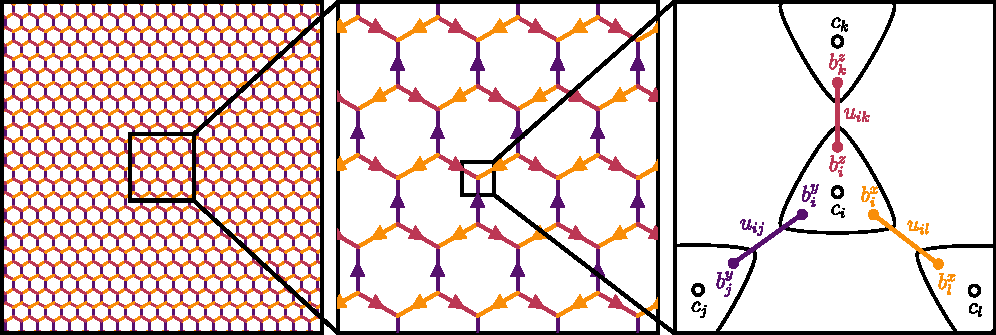
\includegraphics[width=1\textwidth,height=\textheight]{figure_code/amk_chapter/intro/honeycomb_zoom/intro_figure_by_hand}
\caption[{The Kitaev Honeycomb Model}]{\textbf{(a)} The Kitaev honeycomb model is defined on a honeycomb lattice. The special feature of the honeycomb lattice that makes the model solvable is that each vertex is joined by exactly three bonds, i.e.~the lattice is trivalent. One of three labels is assigned to each bond (x,y,z) here represented by colour. \textbf{(b)}. After transforming to the Majorana representation we get an emergent gauge degree of freedom \(u_{jk} = \pm 1\) that lives on each bond, the bond variables. These are antisymmetric, \(u_{jk} = -u_{kj}\), so we represent them graphically with arrows on each bond that point in the direction that \(u_{jk} = +1\) \textbf{(c)}. The Majorana transformation can be visualised as breaking each spin into four Majoranas \(b_i^x,\;b_i^y,\;b_i^z,\;c_i\). The x, y and z Majoranas then pair along the bonds forming conserved \(\mathbb{Z}_2\) bond operators \(u_{jk} = \langle i b_i^\alpha b_j^\alpha \rangle\). The remaining \(c_i\) operators form an effective quadratic Hamiltonian \(H = \frac{i}{4} \sum_{\langle i,j\rangle_\alpha} 2J^{\alpha} u_{ij} \hat{c}_i \hat{c}_j\).}
\label{fig:intro_figure_by_hand}
\end{figure}
}

\hypertarget{the-spin-hamiltonian}{%
\subsection{The Spin Hamiltonian}\label{the-spin-hamiltonian}}

This section introduces the Kitaev honeycomb (KH) model. The KH model is an exactly solvable model of interacting spin\(-1/2\) spins on the vertices of a honeycomb lattice. Each bond in the lattice is assigned a label \(\alpha \in \{ x, y, z\}\) and that bond couple two spins along the \(\alpha\) axis. See \cref{fig:intro_figure_by_hand} for a diagram of the setup.

This gives us the Hamiltonian \begin{equation}\protect\hypertarget{eq:bg-kh-model}{}{ H =  - \sum_{\langle j,k\rangle_\alpha} J^{\alpha}\sigma_j^{\alpha}\sigma_k^{\alpha}, }\label{eq:bg-kh-model}\end{equation} where \(\sigma^\alpha_j\) is the \(\alpha\) component of a Pauli matrix acting on site \(j\) and \(\langle j,k\rangle_\alpha\) is a pair of nearest-neighbour indices connected by an \(\alpha\)-bond with exchange coupling \(J^\alpha\). Kitaev introduced this model in his seminal 2006 paper~\autocite{kitaevAnyonsExactlySolved2006}.

The KH can arise as the result of strong spin-orbit couplings in, for example, the transition metal based compounds~\autocite{Jackeli2009,HerrmannsAnRev2018,Winter2017,TrebstPhysRep2022,Takagi2019}. The model is highly frustrated: each spin would like to align along a different direction with each of its three neighbours but this cannot be achieved even classically~\autocite{chandraClassicalHeisenbergSpins2010,selaOrderbydisorderSpinorbitalLiquids2014}. This frustration leads the model to have a quantum spin liquid (QSL) ground state, a complex many body state with a high degree of entanglement but no long range magnetic order even at zero temperature. While the possibility of a QSL ground state was suggested much earlier~\autocite{andersonResonatingValenceBonds1973}, the KH model was the first exactly solvable models of the QSL state. The KH model has a rich ground state phase diagram with gapless and gapped phases, the latter supporting fractionalised quasiparticles with both Abelian and non-Abelian quasiparticle excitations. Anyons have been the subject of much attention because, among other reasons, they can be braided through spacetime to achieve noise tolerant quantum computations~\autocite{freedmanTopologicalQuantumComputation2003}. At finite temperature the KH model undergoes a phase transition to a thermal metal state~\autocite{selfThermallyInducedMetallic2019}. The KH model can be solved exactly via a mapping to Majorana fermions. This mapping yields an extensive number of static \(\mathbb Z_2\) fluxes tied to an emergent gauge field with the remaining fermions are governed by a free fermion hamiltonian.

This section will go over the standard model in detail, first discussing \protect\hyperlink{the-spin-model}{the spin model}, then detailing the transformation to a \protect\hyperlink{the-majorana-model}{Majorana hamiltonian} that allows a full solution while enlarging the Hamiltonian. We will discuss the properties of the \protect\hyperlink{an-emergent-gauge-field}{emergent gauge fields} and the projector. The \protect\hyperlink{sec:anyons}{next section} will discuss anyons, topology and the Chern number, using the Kitaev model as an explicit example of these topics. Finally will then discuss the ground state found via Lieb's theorem as well as work on generalisations of the ground state to other lattices. Finally we will look at the \protect\hyperlink{ground-state-phases}{phase diagram}.

\hypertarget{the-spin-model}{%
\subsection{The Spin Model}\label{the-spin-model}}

\hypertarget{fig:visual_kitaev_1}{%
\begin{figure}
\centering
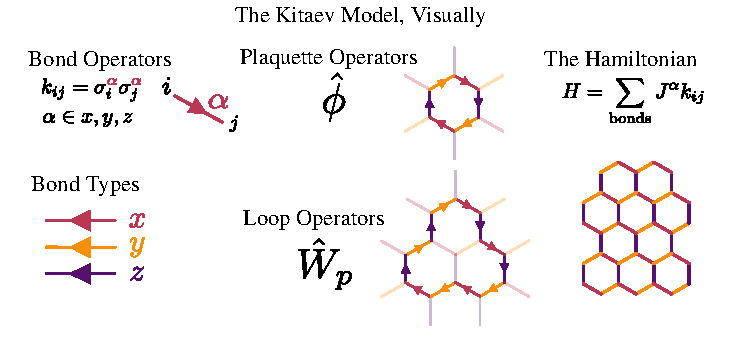
\includegraphics[width=1\textwidth,height=\textheight]{figure_code/amk_chapter/visual_kitaev_1}
\caption[{A Visual Intro to the Kitaev Model}]{A visual introduction to the Kitaev Model.}
\label{fig:visual_kitaev_1}
\end{figure}
}

As discussed in the introduction, spin hamiltonians like that of the Kitaev model arise in electronic systems as the result the balance of multiple effects~\autocite{TrebstPhysRep2022}. For instance, in certain transition metal systems with \(d^5\) valence electrons, crystal field and spin-orbit couplings conspire to shift and split the \(d\) orbitals into moments with spin \(j = 1/2\) and \(j = 3/2\). Of these, the bandwidth \(t\) of the \(j= 1/2\) band is small, meaning that even relatively meagre electron correlations (such those induced by the \(U\) term in the Hubbard model) can lead to the opening of a Mott gap. From there we have a \(j = 1/2\) Mott insulator whose effective spin-spin interactions are again shaped by the lattice geometry and spin-orbit coupling leading some materials to have strong bond-directional Ising-type interactions~\autocite{jackeliMottInsulatorsStrong2009,khaliullinOrbitalOrderFluctuations2005}. In the Kitaev Model the bond directionality refers to the fact that the coupling axis \(\alpha\) in terms like \(\sigma_j^{\alpha}\sigma_k^{\alpha}\) is strongly bond dependent.

In the spin hamiltonian \cref{eq:bg-kh-model} we can already tease out a set of conserved fluxes that will be key to the model's solution. These fluxes are the expectations of Wilson loop operators

\[\hat{W}_p = \prod_{\langle i,j\rangle_\alpha\; \in\; p} \sigma_i^{\alpha}\sigma_j^{\alpha},\]

the products of bonds winding around a closed path \(p\) on the lattice. These operators commute with the Hamiltonian and so have no time dynamics. The winding direction does not matter so long as it is fixed. By convention we will always use clockwise. Each closed path on the lattice is associated with a flux. The number of conserved quantities grows linearly with system size and is thus extensive, this is a common property for exactly solvable systems and can be compared to the heavy electrons present in the Falicov-Kimball model. The square of two loop operators is one so any contractible loop can be expressed as a product of loops around plaquettes of the lattice, as in \cref{fig:stokes_theorem}. For the honeycomb lattice the plaquettes are the hexagons. The expectations of \(\hat{W}_p\) through each plaquette, the fluxes, are therefore enough to describe the whole flux sector. We will focus on these fluxes, denoting them by \(\phi_i\). Once we have made the mapping to the Majorana Hamiltonian I will explain how these fluxes can be connected to an emergent \(B\) field which makes their interpretation as fluxes clear.

\hypertarget{fig:stokes_theorem}{%
\begin{figure}
\centering
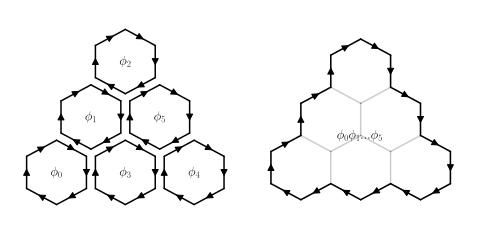
\includegraphics[width=0.71\textwidth,height=\textheight]{figure_code/amk_chapter/stokes_theorem/stokes_theorem}
\caption[{We can construct arbitrary loops from plaquette fluxes.}]{In the Kitaev Honeycomb model, Wilson loop operators \(\hat{W}_p = \prod_{\langle i,j\rangle_\alpha\; \in\; p} \sigma_i^{\alpha}\sigma_j^{\alpha}\) can be composed via multiplication to produce arbitrary contractible loops. As a consequence we need only to keep track of the value of the flux through each plaquette \(\phi_i\). This relationship between the \(u_{ij}\) around a region and fluxes with one is evocative of Stokes' theorem for classical electromagnetism. In fact it turns out to be the exponential of it as we shall make explicit later.}
\label{fig:stokes_theorem}
\end{figure}
}

It is worth noting in passing that the effective Hamiltonian for many Kitaev materials incorporates a contribution from an isotropic Heisenberg term \(\sum_{i,j} \vec{\sigma}_i\cdot\vec{\sigma}_j\), this is referred to as the Heisenberg-Kitaev Model~\autocite{Chaloupka2010}. Materials for which the Kitaev term dominates are generally known as Kitaev Materials. See~\autocite{TrebstPhysRep2022} for a full discussion of Kitaev Materials.

As with the Falicov-Kimball model, the KH model has a extensive number of conserved quantities, the fluxes. As with the FK model it will make sense to work in the simultaneous eigenbasis of the fluxes and the Hamiltonian so that we can treat the fluxes like a classical degree of freedom. This is part of what makes the model tractable. We will find that the ground state of the model corresponds to some particular choice of fluxes. We will refer to local excitations away from the flux ground state as \emph{vortices}. In order to fully solve the model however, we must first move to a Majorana picture.

\hypertarget{the-majorana-model}{%
\subsection{The Majorana Model}\label{the-majorana-model}}

Majorana fermions are something like `half of a complex fermion' and are their own antiparticle. From a set of \(N\) fermionic creation \(f_i^\dagger\) and anhilation \(f_i\) operators we can construct \(2N\) Majorana operators \(c_m\). We can do this construction in multiple ways subject to only mild constraints required to keep the overall commutations relations correct~\autocite{kitaevAnyonsExactlySolved2006}. Majorana operators square to one but otherwise have standard fermionic commutation relations.

\(N\) spins can be mapped to \(N\) fermions with the well known Jordan-Wigner transformation and indeed this approach can be used to solve the Kitaev model~\autocite{chenExactResultsKitaev2008}. Here I will introduce the method Kitaev used in the original paper as this forms the basis for the results that will be presented in this thesis. Rather than mapping to \(N\) fermions, Kitaev maps to \(4N\) Majoranas, effectively \(2N\) fermions. In contrast to the Jordan-Wigner approach which makes fermions out of strings of spin operators in order to correctly produce fermionic commutation relations, the Kitaev transformation maps each spin locally to four Majoranas. The downside is that this enlarges the Hilbert space from \(2^N\) to \(4^N\). We will have to employ a projector \(\hat{P}\) to come back down to the physical Hilbert space later. As everything is local, I will drop the site indices \(ijk\) in expressions that refer to only a single site.

The mapping is defined in terms of four Majoranas per site \(b_i^x,\;b_i^y,\;b_i^z,\;c_i\) such that

\begin{equation}\protect\hypertarget{eq:bg-kh-mapping}{}{\tilde{\sigma}^x = i b^x c,\; \tilde{\sigma}^y = i b^y c,\; \tilde{\sigma}^z = i b^z c}\label{eq:bg-kh-mapping}\end{equation}

The tildes on the spin operators \(\tilde{\sigma_i^\alpha}\) emphasis that they live in this new extended Hilbert space and are only equivalent to the original spin operators after applying a projector \(\hat{P}\). The form of the projection operator can be understood in a few ways. From a group-theoretic perspective, before projection, the operators \(\{\tilde{\sigma}^x, \tilde{\sigma}^y, \tilde{\sigma}^z\}\) form a representation of the gamma group \(G_{3,0}\). The gamma groups \(G_{p,q}\) have \(p\) generators that square to the identity and \(q\) that square (roughly) to \(-1\). The generators otherwise obey standard anticommutation relations. The well known gamma matrices \(\{\gamma^0, \gamma^1, \gamma^2, \gamma^3\}\) represent \(G_{1,3}\) the quaternions \(G_{0,3}\) and the Pauli matrices \(G_{3,0}\).

The Pauli matrices, however, have the additional property that the \emph{chiral element} \(\sigma^x \sigma^y \sigma^z = \pmi\) is not fully determined by the group properties of \(G_{3,0}\) but it is equal to \(i\) in the Pauli matrices. Therefore to fully reproduce the algebra of the Pauli matrices we must project into the subspace where \(\tilde{\sigma}^x \tilde{\sigma}^y \tilde{\sigma}^z = +i\). The chiral element of the gamma matrices for instance \(\gamma_5 = i\gamma^0 \gamma^1 \gamma^2 \gamma^3\) is of central importance in quantum field theory. See~\autocite{petitjeanChiralityDiracSpinors2020} for more discussion of this group theoretic view.

So the projector must project onto the subspace where \(\tilde \sigma^x \tilde \sigma^y \tilde \sigma^z = i\). If we work this through we find that in general \(\tilde \sigma^x \tilde \sigma^y \tilde\sigma^z = iD\) where \(D = b^x b^y b^z c\) must be the identity for every site. In other words, we can only work with \emph{physical states} \(|\phi\rangle\) that satisfy \(D_i|\phi\rangle = |\phi\rangle\) for all sites \(i\). From this we construct an on-site projector \(P_i = \frac{1 + D_i}{2}\) and the overall projector is simply \(P = \prod_i P_i\).

Another way to see what this is doing physically is to explicitly construct the two intermediate fermionic operators \(f\) and \(g\) that give rise to these four Majoranas. Denoting a fermion state by \(|n_f, n_g\rangle\) the Hilbert space is the set \(\{|00\rangle,|01\rangle,|10\rangle,|11\rangle\}\). We can map these to Majoranas with, for example, this definition

\[\begin{aligned}
b^x = (f + f^\dagger),\;\;& b^y = -i(f - f^\dagger),\\
b^z = (g + g^\dagger),\;\;& c = -i(g - g^\dagger),
\end{aligned}\]

Working through the algebra we see that the operator \(D = b^x b^y b^z c\) is equal to the fermion parity \(D = -(2n_f - 1)(2n_g - 1) = \pm1\) where \(n_f,\; n_g\) are the number operators. So setting \(D = 1\) everywhere is equivalent to restricting to the \(\{|01\rangle,|10\rangle\}\) though we could equally well have used the other one.

Expanding the product \(\prod_i P_i\) out, we find that the projector corresponds to a symmetrisation over \(\{u_{ij}\}\) states within a flux sector and and overall fermion parity \(\prod_i D_i\). The significance of this is that an arbitrary many body state can be made to have non-zero overlap with the physical subspace via the addition or removal of just a single fermion. This implies that in the thermodynamic limit the projection step is not generally necessary to extract physical results, see~\autocite{pedrocchiPhysicalSolutionsKitaev2011} or \protect\hyperlink{app-the-projector}{appendix A.5} for more details.

We can now rewrite the spin hamiltonian in Majorana form with the caveat that they are only strictly equivalent after projection. The Ising interactions \(\sigma_j^{\alpha}\sigma_k^{\alpha}\) decouple into the form \(-i (i b^\alpha_i b^\alpha_j) c_i c_j\). We factor out the \emph{bond operators} \(\hat{u}_{ij} = i b^\alpha_i b^\alpha_j\) which are Hermitian and, remarkably, commute with the Hamiltonian and each other.

\[\begin{aligned}
\tilde{H} &=  - \sum_{\langle i,j\rangle_\alpha} J^{\alpha}\tilde{\sigma}_i^{\alpha}\tilde{\sigma}_j^{\alpha}\\
          &=  i \sum_{\langle i,j\rangle_\alpha} J^{\alpha} \hat{u}_{ij} \hat{c}_i \hat{c}_j
\end{aligned}\]

The bond operators \(\hat{u}_{ij}\) square to one so have eigenvalues \(\pm1\). As they're conserved we will work in their eigenbasis and take off the hats in the Hamiltonian.

\begin{equation}\protect\hypertarget{eq:bg-kh-maj-model}{}{\begin{aligned}
H &=  i \sum_{\langle i,j\rangle_\alpha} J^{\alpha} u_{ij} \hat{c}_i \hat{c}_j
\end{aligned}}\label{eq:bg-kh-maj-model}\end{equation}

\hypertarget{the-fermion-problem}{%
\subsection{The Fermion Problem}\label{the-fermion-problem}}

We now have a quadratic Hamiltonian, \cref{eq:bg-kh-maj-model}, coupled to a classical field \(u_{ij}\). What follows is relatively standard theory for quadratic Hamiltonians~\autocite{BlaizotRipka1986}.

Because of the antisymmetry \(J^{\alpha} u_{ij}\), the eigenvalues of \cref{eq:bg-kh-maj-model} come in pairs \(\pm \epsilon_m\). We organise the eigenmodes of \(H\) into pairs, such that \(b_m\) and \(b_m'\) have energies \(\epsilon_m\) and \(-\epsilon_m\). The transformation \(Q\)

\[(c_1, c_2... c_{2N}) Q = (b_1, b_1', b_2, b_2' ... b_{N}, b_{N}')\]

puts the Hamiltonian into normal mode form

\[H = \frac{i}{2} \sum_m \epsilon_m b_m b_m'.\]

The determinant of \(Q\) appears when evaluating the projector explicitly, otherwise, the \(b_m\) are merely an intermediate step. From them, we form fermionic operators

\[ f_i = \tfrac{1}{2} (b_m + ib_m')\]

with their associated number operators \(n_i = f^\dagger_i f_i\). These let us write the Hamiltonian neatly as

\[ H = \sum_m \epsilon_m (n_m - \tfrac{1}{2}).\]

The energy of the ground state \(|n_m = 0\rangle\) of the many body system at fixed \(\{u_{ij}\}\) is

\[E_{0} = -\frac{1}{2}\sum_m \epsilon_m \]

and we can construct any state from a particular choice of \(n_m = 0,1\). If we only care about the ground state energy \(E_{0}\), it is possible to skip forming the fermionic operators. The eigenvalues obtained directly from diagonalising \(J^{\alpha} u_{ij}\) come in \(\pm \epsilon_m\) pairs. We can take half the absolute value of the set to recover \(\sum_m \epsilon_m\) directly.

\hypertarget{an-emergent-gauge-field}{%
\subsection{An Emergent Gauge Field}\label{an-emergent-gauge-field}}

We have transformed the spin Hamiltonian into a Majorana hamiltonian \(H = i \sum_{\langle i,j\rangle_\alpha} J^{\alpha} u_{ij} \hat{c}_i \hat{c}_j\) describing the dynamics of a classical field \(u_{ij}\) and Majoranas \(c_i\). It is natural to ask how the classical field \(u_{ij}\) relates to the fluxes of the original spin model. We can evaluate the fluxes \(\phi_i\) in terms of the bond operators

\begin{equation}\protect\hypertarget{eq:flux-majorana}{}{\phi_i = \prod_{\langle j,k\rangle \in \mathcal{P}_i} i u_{jk}.}\label{eq:flux-majorana}\end{equation}

\hypertarget{fig:gauge_symmetries}{%
\begin{figure}
\centering
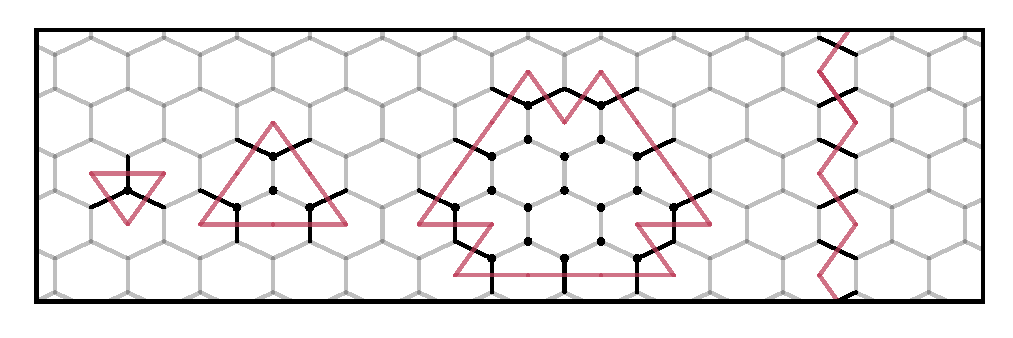
\includegraphics[width=1\textwidth,height=\textheight]{figure_code/amk_chapter/intro/gauge_symmetries/gauge_symmetries}
\caption[{Gauge Symmetries}]{A honeycomb lattice with edges in light grey, along with its dual, the triangle lattice in light blue. The vertices of the dual lattice are the faces of the original lattice and, hence, are the locations of the vortices. (Left) The action of the gauge operator \(D_j\) at a vertex is to flip the value of the three \(u_{jk}\) variables (black lines) surrounding site \(j\). The corresponding edges of the dual lattice (red lines) form a closed triangle. (Middle) Composing multiple adjacent \(D_j\) operators produces a large closed dual loop or multiple disconnected dual loops. Dual loops are not directed like Wilson loops. (Right) A non-contractable loop which cannot be produced by composing \(D_j\) operators. All three operators can be thought of as the action of a vortex-vortex pair that is created, one of them is transported around the loop, and then the two annihilate again. Note that every plaquette has an even number of \(u_{ij}\)s flipped on its edge. Therefore, all retain the same flux \(\phi_i\).}
\label{fig:gauge_symmetries}
\end{figure}
}

In addition, the bond operators form a highly degenerate description of the system. The operators \(D_i = b^x_i b^y_i b^z_i c_i\) commute with \(H\) forming a set of local symmetries. The action of \(D_i\) on a state is to flip the values of the three \(u_{ij}\) bonds that connect to site \(i\). This changes the bond configuration \(\{u_{ij}\}\) but leaves the flux configuration \(\{\phi_i\}\) unchanged. Physically, we interpret \(u_{ij}\) as a gauge field with a high degree of degeneracy and \(\{D_i\}\) as the set of gauge symmetries. The Majorana bond operators \(u_{ij}\) are an emergent, classical, \(\mathbb{Z}_2\) gauge field! The flux configuration \(\{\phi_i\}\) is what encodes physical information about the system without all the gauge degeneracy.

The ground state of the Kitaev Honeycomb model is the all one flux configuration \(\{\phi_i = +1\; \forall \; i\}\). This can be proven via Lieb's theorem~\autocite{lieb_flux_1994} which gives the lowest energy magnetic flux configuration for a system of electrons hopping in a magnetic field. Kitaev remarks in his original paper that he was not initially aware of the relevance of Lieb's 1994 result. This is not surprising because at first glance the two models seem quite different but the connection is quite instructive for understanding the Kitaev Model and its generalisations.

Lieb discusses a model of mobile electrons

\[H = \sum_{ij} t_{ij} c^\dagger_i c_j\]

where the hopping terms \(t_{ij} = |t_{ij}|\exp(i\theta_{ij})\) incorporate Aharanhov-Bohm (AB) phases~\autocite{aharonovSignificanceElectromagneticPotentials1959} \(\theta_{ij}\). The AB phases model the effect of a slowly varying magnetic field on the electrons through the integral of the magnetic vector potential \(\theta_{ij} = \int_i^j \vec{A} \cdot d\vec{l}\), a Peierls substitution~\autocite{peierlsZurTheorieDiamagnetismus1933}. If we map the Majorana form of the Kitaev model to Lieb's model we see that our \(t_{ij} = i J^\alpha u_{ij}\). The \(i u_{ij} = \pm i\) correspond to AB phases \(\theta_{ij} = \pi/2\) or \(3\pi/2\) along each bond.

\hypertarget{fig:regular_plaquettes}{%
\begin{figure}
\centering
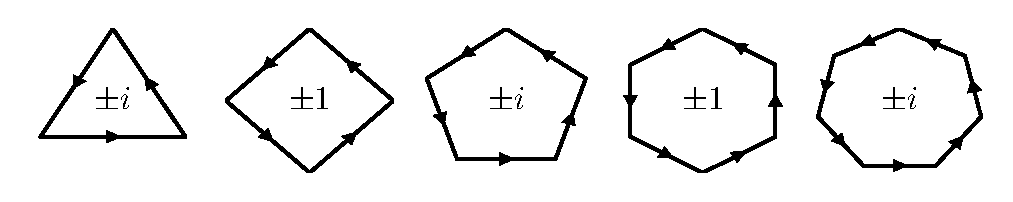
\includegraphics[width=0.86\textwidth,height=\textheight]{figure_code/amk_chapter/intro/regular_plaquettes/regular_plaquettes}
\caption[{Plaquettes in the Kitaev Model}]{Lieb's theorem gives the ground state flux configuration for even sided plaquettes in systems with at least one translationally invariant direction~\autocite{lieb_flux_1994}. These labels correspond to the Kitaev fluxes \(\phi_i\) rather than the magnetic fluxes \(Q_i\) of Lieb's original paper (\(\phi_i = \exp{iQ_i}\)). Other work has extended Lieb's theorem numerically to arbitrary plaquettes,~\autocite{eschmannThermodynamicClassificationThreedimensional2020,Yao2009,eschmann2019thermodynamics,Peri2020}. The additional twofold degeneracy of the \(\pm i, \mp i\) terms is a consequence of the odd sided plaquettes breaking chiral symmetry. Chiral symmetry is spontaneously broken in the ground state~\autocite{Yao2009}.}
\label{fig:regular_plaquettes}
\end{figure}
}

Stokes' theorem tells us that the magnetic flux \(Q_m\) through a surface \(S\) is related to the line integral of \(\vec{A}\) along the boundary of the surface \(\partial S\) which in the discrete case reduces to the sum of the AB phases along the path. We can thus rewrite \cref{eq:flux-majorana} as

\begin{equation}\protect\hypertarget{eq:flux-magnetic}{}{\begin{aligned}
\phi_i &= \prod_{\mathcal{P}_i} i u_{jk}\\
       &= \prod_{\mathcal{P}_i} \exp{(i\theta_{jk}})\\
       &= \exp \left( i \sum_{\mathcal{P}_i} \theta_{jk} \right)\\
       &= \exp \left( i \oint_{\mathcal{P}_i} \vec{A} \cdot d\vec{l} \right)\\
       &= \exp \left( i Q_i \right)
\end{aligned}}\label{eq:flux-magnetic}\end{equation}

Thus we can interpret the fluxes \(\phi_i\) as the exponential of magnetic fluxes \(Q_m\) of some fictitious gauge field \(\vec{A}\) and the bond operators as \(i u_{ij} = \exp i \int_i^j \vec{A} \cdot d\vec{l}\). In this analogy to classical electromagnetism, the sets \(\{u_{ij}\}\) that correspond to the same \(\{\phi_i\}\) are all gauge equivalent as we have already seen via other means. The fact that fluxes can be written as products of bond operators and composed is a consequence of \cref{eq:flux-magnetic}. If the lattice contains odd plaquettes, as in the Yao-Kivelson model~\autocite{yaoExactChiralSpin2007}, the complex fluxes that appear are a sign that chiral symmetry has been broken.

In full, Lieb's theorem states that the ground state has magnetic flux \(Q_i = \sum_{\mathcal{P}_i}\theta_{ij} = \pi \; (\mathrm{mod} \;2\pi)\) for plaquettes with \(0 \; (\mathrm{mod}\;4)\) sides and \(0 \; (\mathrm{mod}\;2\pi)\) for plaquettes with \(2 \; (\mathrm{mod}\;4)\) sides. In terms of our fluxes, this means \(\phi = -1\) for squares, \(\phi = 1\) for hexagons and so on.

While Lieb's theorem is restricted to bipartite lattices with translational symmetry, other works has shown numerically that it tends to hold for more general lattices too~\autocite{eschmannThermodynamicClassificationThreedimensional2020,Yao2009,eschmann2019thermodynamics,Peri2020}. From this we find that the generalisation to odd sided plaquettes is similar but with an additional chiral symmetry, so \(\phi = \pm i\) for plaquettes with \(1 \; (\mathrm{mod}\;4)\) sides and \(\mp i\) for those with \(3 \; (\mathrm{mod}\;4)\) sides. Overall we can write \(\phi = -(\pm i)^{n_{\mathrm{sides}}}\). Later I will present numerical evidence that this rule continues to hold for general amorphous lattices.

Understanding \(u_{ij}\) as a gauge field provides another way to understand the action of the projector. The local projector \(P_i = \frac{1 + D_i}{2}\) applied to a state constructs a superposition of the original state and the gauge equivalent state linked to it by flipping the three \(u_{ij}\) around site \(i\). The overall projector \(P = \prod_i P_i\) can thus be understood as a symmetrisation over all gauge equivalent states, removing the gauge degeneracy introduced by the mapping from spins to Majoranas.

\hypertarget{fig:topological_fluxes}{%
\begin{figure}
\centering
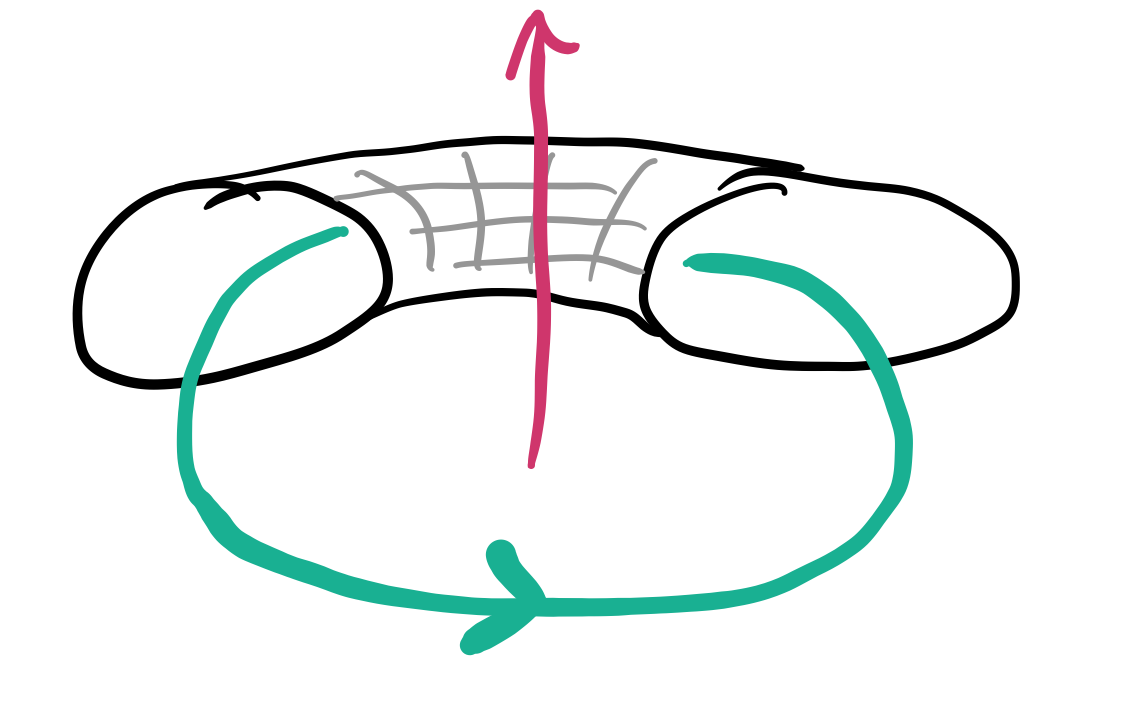
\includegraphics[width=0.57\textwidth,height=\textheight]{figure_code/amk_chapter/topological_fluxes.png}
\caption[{Topological Fluxes}]{Wilson loops that wind the major or minor diameters of the torus measure flux winding through the hole of the doughnut/torus (red) or through the filling (green). If they made doughnuts which had both had a jam filling and a hole, this analogy would be a lot easier to make~\autocite{parkerWhyDoesThis}.}
\label{fig:topological_fluxes}
\end{figure}
}

A final but important point to mention is that the local fluxes \(\phi_i\) are not quite all there is. We've seen that products of \(\phi_i\) can be used to construct the flux associated with arbitrary contractible loops. On the plane contractible loops are all there is. However, on the torus we can construct two global fluxes \(\Phi_x\) and \(\Phi_y\) which correspond to paths tracing the major and minor axes. The four sectors spanned by the \(\pm1\) values of these fluxes are gapped away from one another but only by virtual tunnelling processes so the gap decays exponentially with system size~\autocite{kitaevAnyonsExactlySolved2006}. Physically \(\Phi_x\) and \(\Phi_y\) could be thought of as measuring the flux that threads through the hole of the doughnut. In general, surfaces with genus \(g\) have \(g\) `handles' and \(2g\) of these global fluxes. At first glance it may seem this would not have much relevance to physical realisations of the Kitaev model that will likely have a planar geometry with open boundary conditions. However these fluxes are closely linked to topology and the existence of anyonic quasiparticle excitations in the model, which we will discuss next.

\hypertarget{sec:anyons}{%
\subsection{Anyons, Topology and the Chern number}\label{sec:anyons}}

\hypertarget{fig:braiding}{%
\begin{figure}
\centering
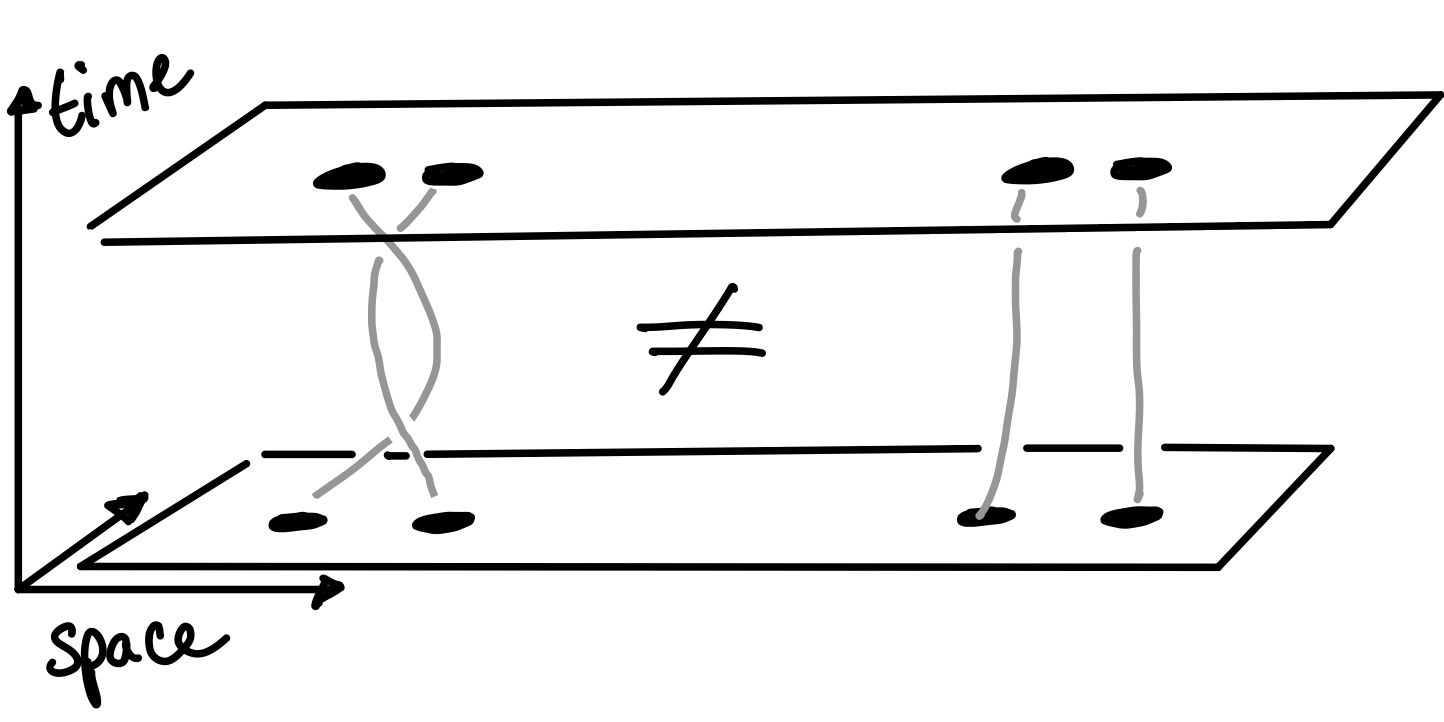
\includegraphics[width=0.71\textwidth,height=\textheight]{figure_code/amk_chapter/braiding.png}
\caption[{Braiding in Two Dimensions}]{Worldlines of particles in two dimensions can become tangled or \emph{braided} with one another.}
\label{fig:braiding}
\end{figure}
}

To discuss different ground state phases of the KH model we must first review the topic of anyons and topology. The standard argument for the existence of Fermions and Bosons goes like this: the quantum state of a system must pick up a factor of \(\pm1\) if two identical particles are swapped. Only \(\pm1\) are allowed since swapping twice must correspond to the identity. This argument works in three dimensions for states without topological degeneracy, which seems to be true of the real world, but condensed matter systems are subject to no such constraints.

In gapped condensed matter systems, all equal time correlators decay exponentially with distance~\autocite{hastingsLiebSchultzMattisHigherDimensions2004}. Put another way, gapped systems support quasiparticles with a definite location in space and finite extent. As such it is meaningful to consider what would happen to the overall quantum state if we were to adiabatically carry out a series of swaps as described above. This is known as braiding. Recently, braiding in topological systems has attracted interest because of proposals to use ground state degeneracy to implement both passively fault tolerant and actively stabilised quantum computations~\autocite{kitaev_fault-tolerant_2003,poulinStabilizerFormalismOperator2005,hastingsDynamicallyGeneratedLogical2021}.

First we realise that in two dimensions, swapping identical particles twice is not topologically equivalent to the identity, see \cref{fig:braiding}. Instead it corresponds to encircling one particle around the other. This means we can in general pick up any complex phase \(e^{i\theta}\), hence the name \textbf{any}-ons upon exchange. These are known as Abelian anyons because complex multiplication commutes and hence the group of braiding operations forms an Abelian group.

The KH model has a topologically degenerate ground state with sectors labelled by the values of the topological fluxes \((\Phi_x\), \(\Phi_y)\). Consider the operation in which a quasiparticle pair is created from the ground state, transported around one of the non-contractible loops and then annihilated together, call them \(\mathcal{T}_{x}\) and \(\mathcal{T}_{y}\). These operations move the system around within the ground state manifold and they need not commute. This leads to non-Abelian anyons. As Kitaev points out, these operations are not specific to the torus: the operation \(\mathcal{T}_{x}\mathcal{T}_{y}\mathcal{T}_{x}^{-1}\mathcal{T}_{y}^{-1}\) corresponds to an operation in which none of the particles crosses the torus, rather one simply winds around the other, hence these effects are relevant even for the planar case.

In condensed matter systems, the existence of anyonic excitations automatically implies the system has topological ground state degeneracy on the torus~\autocite{einarssonFractionalStatisticsTorus1990} and indeed anyons and topology are intimately linked~\autocite{oshikawaTopologicalDegeneracyNonAbelian2007,Chung_Topological_quantum2010,yaoAlgebraicSpinLiquid2009}. The Chern number \(\nu\), a concept originally used to describe complex vector bundles in algebraic topology~\autocite{chernCharacteristicClassesHermitian1946}, has found use in physics as a powerful diagnostic tool for topological systems. Kitaev showed that there is a full classification of anyonic statistics in terms of \(\nu\;(\mathrm{mod}\;16)\) but relevant to us is that vortices in the KH model are Abelian when the Chern number is even and non-Abelian when the Chern number is odd. Non-Abelian statistics of the vortices in the KH model arise due to unpaired Majorana modes that are bound to them.

\hypertarget{ground-state-phases}{%
\subsection{Ground State Phases}\label{ground-state-phases}}

\hypertarget{fig:KH_phase_diagram}{%
\begin{figure}
\centering
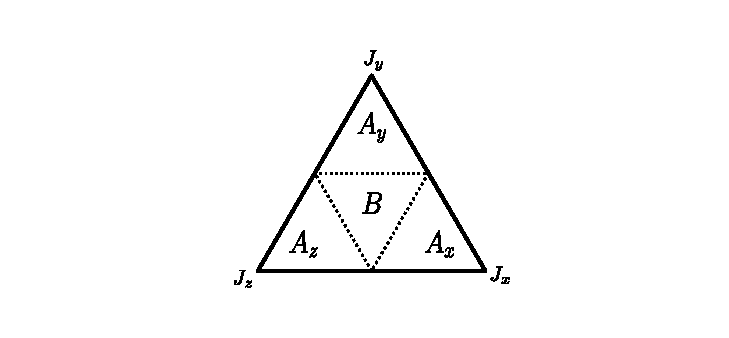
\includegraphics[width=1\textwidth,height=\textheight]{figure_code/background_chapter/KH_phase_diagram}
\caption[{Kitaev Honeycomb Model Phase Diagram}]{Setting the energy scale of the Kitaev Model with the constraint that \(J_x + J_y + J_z = 1\) yields a triangular phase diagram where each of the corners represents \(J_\alpha = 1\). For each corner \(\alpha\) the region \(|J_\alpha > |J_\beta| + |J_\gamma|\) supports a gapped non-Abelian phase equivalent to that of the Toric code~\autocite{kitaev1997quantum,kitaev_fault-tolerant_2003}. The point around equal coupling \(J_x = J_y = J_z\), the B phase, is gapless. The B phase is known a Majorana metal and on the honeycomb lattice it has a Dirac cone dispersion similar to that of graphene.}
\label{fig:KH_phase_diagram}
\end{figure}
}

Setting the overall energy scale with the constraint \(J_x + J_y + J_z = 1\) yields a triangular phase diagram. In each of the corners one of the spin-coupling directions dominates, \(|J_\alpha > |J_\beta| + |J_\gamma|\), yielding three equivalent \(A_\alpha\) phases while the central triangle around \(J_x = J_y = J_z\) is called the B phase. Both phases support two kinds of quasiparticles, fermions and \(\mathbb{Z}_2\)-vortices. In the A phases, the vortices have bosonic statistics with respect to themselves but act like fermions with respect to the fermions, hence they are Abelian anyons, This phase has the same anyonic structure as the Toric code~\autocite{kitaev_fault-tolerant_2003}. The B phase can be described as a semi-metal of the Majorana fermions~\autocite{TrebstPhysRep2022}. Since the B phase is gapless, the quasiparticles aren't localised and so don't have braiding statistics.

An external magnetic can be used to break chiral symmetry. The lowest order term that breaks chiral symmetry but retains the solvability of the model is the three spin term \[
\sum_{(i,j,k)} \sigma_i^{\alpha} \sigma_j^{\beta} \sigma_k^{\gamma}
\] where the sum \((i,j,k)\) runs over consecutive indices around plaquettes. The addition of this to the spin model leads to two bond terms in the corresponding Majorana model. The effect of breaking chiral symmetry is to open a gap in the B phase. The vortices of the gapped B phase are non-Abelian anyons. This phase has the same anyonic exchange statistics as \(p_x + ip_y\) superconductor~\autocite{readPairedStatesFermions2000}, the Moore-Read state for the \(\nu = 5/2\) fractional quantum Hall state~\autocite{mooreNonabelionsFractionalQuantum1991} and many other systems~\autocite{aliceaNonAbelianStatisticsTopological2011,fuSuperconductingProximityEffect2008,lutchynMajoranaFermionsTopological2010,oregHelicalLiquidsMajorana2010,sauGenericNewPlatform2010}. Collectively these systems have attracted interest as possible physical realisations for braiding based quantum computers.

At finite temperatures, recent work has shown that the KH model undergoes a transition to a thermal metal phase.

To surmise, the Kitaev Honeycomb model is remarkable because it combines three key properties. First, the form of the Hamiltonian plausibly be realised by a real material. Candidate materials, such as \(\alpha\mathrm{-RuCl}_3\), are known to have sufficiently strong spin-orbit coupling and the correct lattice structure to behave according to the Kitaev Honeycomb model with small corrections~\autocite{banerjeeProximateKitaevQuantum2016,TrebstPhysRep2022}. Second, its ground state is the canonical example of the long sought after quantum spin liquid state, its dynamical spin-spin correlation functions are zero beyond nearest neighbour separation~\autocite{baskaranExactResultsSpin2007}. Its excitations are anyons, particles that can only exist in two dimensions that break the normal fermion/boson dichotomy.

Third, and perhaps most importantly, this model is a rare many body interacting quantum system that can be treated analytically. It is exactly solvable. We can explicitly write down its many body ground states in terms of single particle states~\autocite{kitaevAnyonsExactlySolved2006}. The solubility of the Kitaev Honeycomb Model, like the Falicov-Kimball model of chapter 1, comes about because the model has extensively many conserved degrees of freedom. These conserved quantities can be factored out as classical degrees of freedom, leaving behind a non-interacting quantum model that is easy to solve.
